\documentclass[11pt,a4paper]{article}
\usepackage[T1]{fontenc}
\usepackage[utf8]{inputenc}
\usepackage{lmodern}
\usepackage[margin=22mm,headheight=16pt]{geometry}
\usepackage{amsmath,amssymb,graphicx,array,longtable,booktabs}
\usepackage{microtype,xcolor,hyperref,xurl,fancyhdr}
\definecolor{Navy}{HTML}{17324D}
\definecolor{Teal}{HTML}{087F8C}
\definecolor{Gold}{HTML}{B88128}
\hypersetup{colorlinks=true,linkcolor=Navy,urlcolor=Teal,bookmarksnumbered=true,hypertexnames=false}
\setlength{\parindent}{0pt}
\setlength{\parskip}{6pt}
\setlength{\emergencystretch}{4em}
\setcounter{tocdepth}{1}
\pagestyle{fancy}\fancyhf{}
\fancyfoot[R]{\small\thepage}
\fancyfoot[L]{\small\sffamily Sharif University of Technology}
\renewcommand{\headrulewidth}{0.3pt}
\makeatletter
\renewcommand\section{\@startsection{section}{1}{\z@}{-3.2ex plus -1ex minus -.2ex}{1.6ex plus .2ex}{\normalfont\Large\sffamily\bfseries\color{Navy}}}
\renewcommand\subsection{\@startsection{subsection}{2}{\z@}{-2.5ex plus -1ex minus -.2ex}{1.2ex plus .2ex}{\normalfont\large\sffamily\bfseries\color{Teal}}}
\makeatother
\fancyhead[L]{\small\sffamily\color{Navy}Sharif University of Technology}\fancyhead[R]{\small\sffamily\color{Teal}Project Assignment}\begin{document}
\begin{titlepage}\centering\vspace*{7mm}

\includegraphics[width=31mm]{assets/sharif_emblem_en.png}\par\vspace{5mm}
{\Large\sffamily\bfseries\color{Navy}SHARIF UNIVERSITY OF TECHNOLOGY\par}
\vspace{2mm}{\sffamily Department of Electrical Engineering\par}
\vspace{17mm}{\color{Teal}\rule{\linewidth}{1.4pt}}\par\vspace{6mm}
{\large\sffamily\color{Teal}PROJECT ASSIGNMENT\par}
\vspace{8mm}{\huge\sffamily\bfseries\color{Navy}RDD Streaming, Cardinality Sketches, and PageRank Algorithms\par}
\vspace{9mm}{\color{Gold}\rule{45mm}{1pt}}\par\vfill
\begin{minipage}{.88\linewidth}
{\sffamily\color{Teal}INSTRUCTOR / INSTRUCTORS}\par
Dr Iman Gholampour\par\vspace{7mm}
{\sffamily\color{Teal}ACADEMIC CONTEXT}\par
Big Data Processing\par\end{minipage}\vfill
\end{titlepage}
\tableofcontents\clearpage
\section{Theory exercise 1: ranking a four-page directed graph}

For the graph supplied in the fourth Big Data Analytics assignment, write its transition matrix, giving the probability from each page to each outgoing neighbor. Use beta=\allowbreak{}0.85 when needed. Compute topic-sensitive PageRank with teleport to A alone, then equally to A/\allowbreak{}C, and explain rank changes. With B as the trusted page, compute TrustRank and Spam Mass and discuss suspicious pages. Compute HITS authority/\allowbreak{}hub scores and explain whether high authority implies high PageRank. Preserve the original graph figure with these questions.

\section{Theory exercise 2: DGIM}

Process S=\allowbreak{}1011101101111011 in chronological order with window N=\allowbreak{}12. Show all bucket merges, final sizes/\allowbreak{}timestamps, and time coverage. Estimate the number of ones in the last K=\allowbreak{}7 bits. Compare with the true count and calculate absolute/\allowbreak{}relative error.

\section{Theory exercise 3: Flajolet-Martin}

For 001011000,100100000,010010000,110111000,000001000,101000000 compute trailing-zero counts and R=\allowbreak{}max r(a). Estimate distinct cardinality with 2\textasciicircum{}R. Add 000000000 and compute the new R. Explain why an additional element need not improve the estimate, and discuss under/\allowbreak{}overestimation when m is much larger/\allowbreak{}smaller than 2\textasciicircum{}R.

\section{Theory exercise 4: partitioned Bloom filter}

An allowed-email set has m entries and n available bits. Divide memory into k arrays and hash once into each. Derive false-positive probability as a function of m,n,k, compare to k hashes in one array, and determine the approximate optimal number of hashes. State the assumptions about uniform independent hashing and equal array sizes.

\section{Theory exercise 5: linked spam farms}

Discuss how two cooperating spam farmers could link their farms to increase target-page PageRank. Explain the proposed structure and any advantage, taking account of outdegree dilution and graph assumptions rather than claiming a universal optimum without specifying the farm model.

\begin{figure}[!htbp]\centering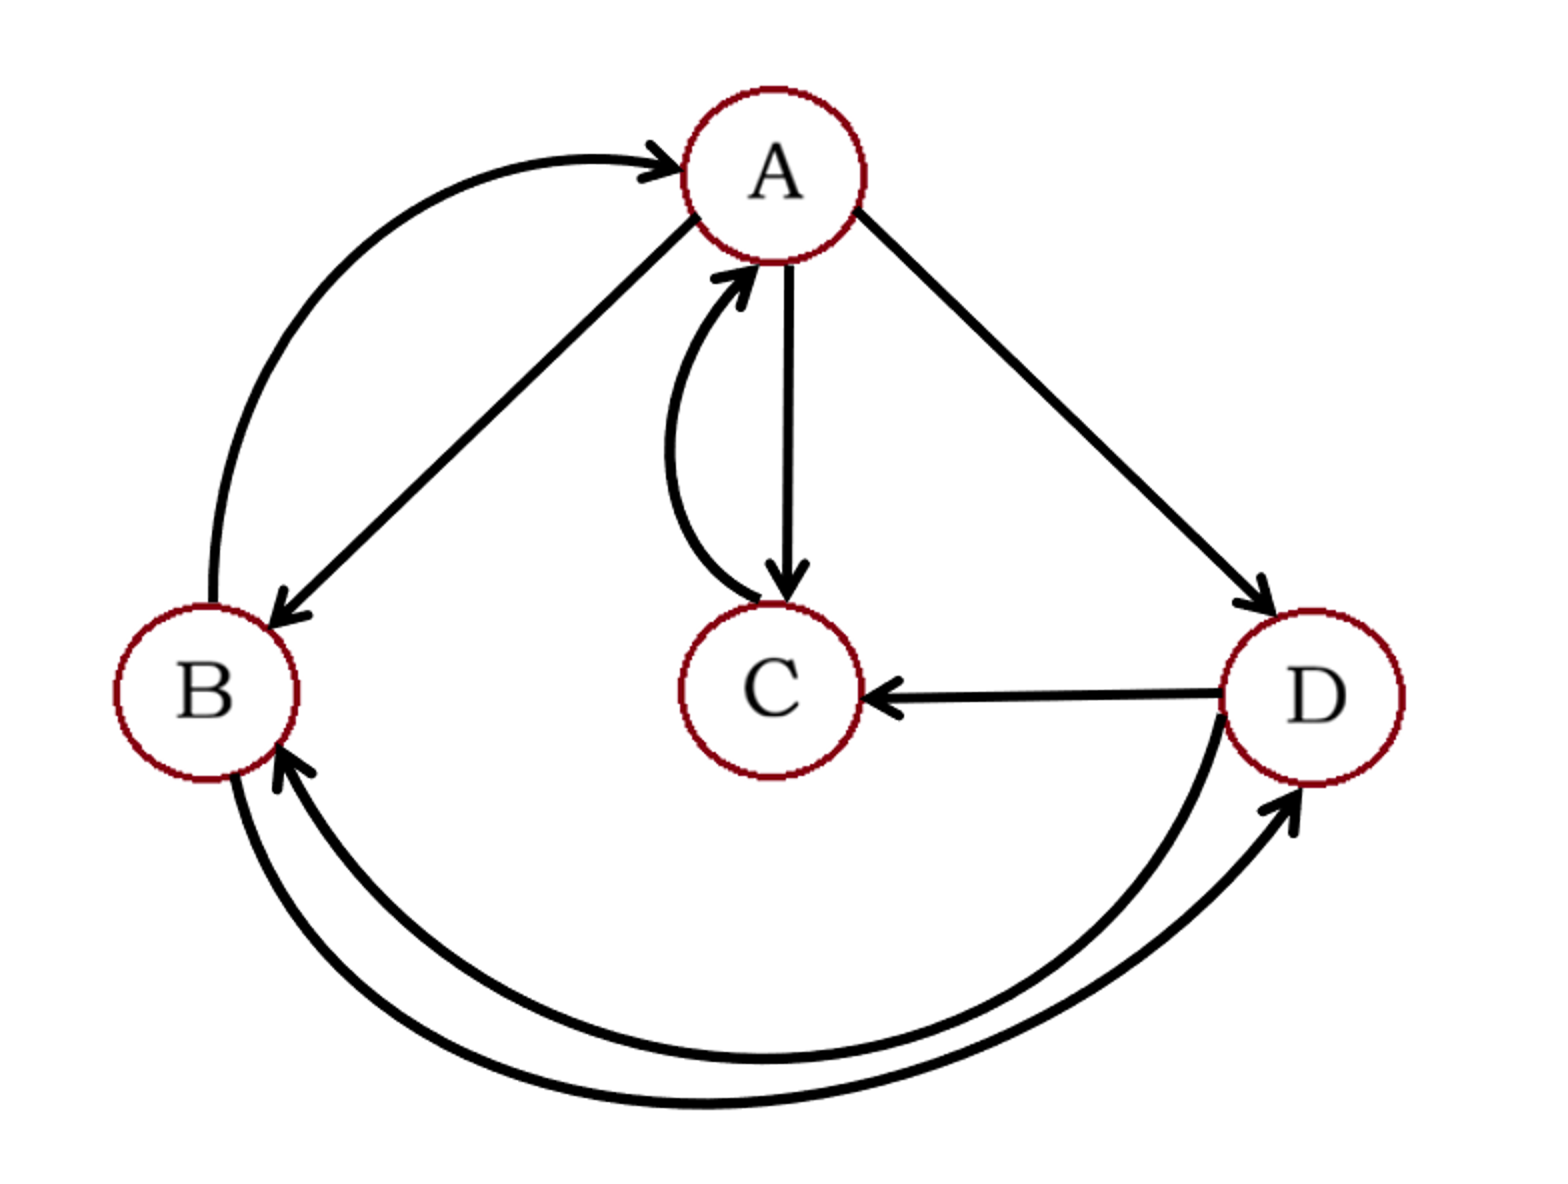
\includegraphics[width=\linewidth,height=.72\textheight,keepaspectratio]{assets/rar_HW4_p002_01.png}\caption{Diagram or recorded result: Theory exercise 5: linked spam farms.}\label{fig:rar_HW4_p002_010}\end{figure}
\clearpage
\section{Practical exercise 1: DStream traffic windows}

Simulate streaming arrival from traffic.csv. Use Spark Streaming DStreams and RDD transformations/\allowbreak{}actions only;\allowbreak{} DataFrames and Structured Streaming are prohibited. Choose and justify window/\allowbreak{}slide durations based on input rate and purpose. Display total passage counts and (DeviceCode,count) by camera for every window. Report the three busiest cameras and explain why windows are needed, the stability/\allowbreak{}responsiveness tradeoff, and the effect of shorter/\allowbreak{}longer windows. Choose a behavioral window and adjustable N;\allowbreak{} report Plate\_\allowbreak{}index values recorded more than N times. Explain the interval and alternatives. For each camera compute distinct plates divided by total records in a selected window. Interpret the ratio cautiously, justify the interval, identify high-count/\allowbreak{}low-diversity cameras, discuss plausible settings, and explain sensitivity to window length. Deliver complete code, analysis, logs, and console screenshots.

\section{Practical exercise 2: probabilistic distinct counting}

The supplied camera-pass stream contains RecordID, CameraID, PlateNumber, RecordTime, Lane, and Speed. Read PlateNumber as a stream. Use hashlib with md5, sha1, sha224, and sha256, convert hashes to binary, and implement trailing-zero-based FM counting. Estimate distinct plates globally and per camera. Report exact distinct counts, estimates, and preferably percentage error. Keep the distinction between cumulative sketches and expiring windows explicit.

\section{Practical exercise 3: traffic PageRank}

Load passages as an RDD, group each plate's observations, and sort by timestamp. Generate a directed edge from the previous camera to the next for each consecutive passage. Show an adjacency-list sample and count nodes/\allowbreak{}edges. Implement iterative PageRank with initial 1/\allowbreak{}N and beta=\allowbreak{}0.85. Identify and correctly handle nodes without outgoing links. Report the ten highest ranks and compare them with the ten highest traffic counts from the previous exercise. Explain what graph structure adds to raw observation totals. Plot a rank-selected subgraph:\allowbreak{} cameras as nodes, observed transitions as directed edges, and line thickness proportional to a clearly defined importance/\allowbreak{}weight. Distinguish event-edge counts from unique camera-pair counts.

\end{document}